\documentclass[aspectratio=169]{beamer}
\usetheme{Madrid}
\usecolortheme{default}

% Modern package imports
\usepackage{graphicx}
\usepackage{tikz}
\usetikzlibrary{shapes, arrows, positioning, calc, shapes.symbols, shapes.geometric, decorations.pathmorphing, backgrounds}
\usepackage{tcolorbox}
\usepackage{xcolor}
\usepackage{amssymb}
\usepackage{booktabs}

% Modern color palette
\definecolor{primaryblue}{RGB}{26,115,232}
\definecolor{accentgreen}{RGB}{34,197,94}
\definecolor{accentorange}{RGB}{251,146,60}
\definecolor{accentpurple}{RGB}{147,51,234}
\definecolor{lightgray}{RGB}{249,250,251}
\definecolor{darkgray}{RGB}{55,65,81}

% Apply modern colors to theme
\setbeamercolor{structure}{fg=primaryblue}
\setbeamercolor{frametitle}{bg=primaryblue!15,fg=primaryblue}
\setbeamercolor{block title}{bg=primaryblue!20,fg=primaryblue}
\setbeamercolor{block body}{bg=lightgray}

% Modern font settings
\setbeamerfont{frametitle}{size=\large,series=\bfseries}
\setbeamerfont{block title}{size=\normalsize,series=\bfseries}

% Logo configuration for title page (update path and positioning as needed)
% Place your institute logo file (logo.jpeg) in the same directory as this .tex file

% Modern footer - clean and minimal
\setbeamertemplate{footline}{
  \leavevmode%
  \hbox{%
  \begin{beamercolorbox}[wd=1\paperwidth,ht=3ex,dp=1.5ex,right]{date in head/foot}%
    \usebeamerfont{footline}\color{darkgray}
    \hspace*{2em}
    \insertframenumber{} / \inserttotalframenumber
    \hspace*{2em}
  \end{beamercolorbox}}%
  \vskip0pt%
}
\setbeamertemplate{navigation symbols}{}  % Remove navigation symbols
\setbeamercolor{date in head/foot}{fg=darkgray}

\title[AI-Powered DBMS]{AI-Powered Database Management System}
\subtitle{A Full-Stack Application for Natural Language to SQL Conversion}
\author[Ankit, Rineet]{123CS0011 - Ankit Kumar \and 123CS0009 - Rineet Pandey}
\institute[Institute]{Department of Computer Science}
\date{\today}

\begin{document}

% Title Slide with Institute Logo
\begin{frame}[plain]
    \begin{tikzpicture}[remember picture, overlay]
        % Institute logo positioned at very top center
        % Shifted higher to avoid overlap with blue title box
        % To adjust position: change yshift (vertical offset from top edge)
        % To adjust size: change height value
        % To use different file: change logo.jpeg to your file name
        \node[anchor=north, yshift=-0.2cm] at (current page.north) {
            \includegraphics[height=1.5cm]{logo.jpeg}
        };
    \end{tikzpicture}
    
    % Add space to push title box down, avoiding logo overlap
    \vspace{2.2cm}
    \titlepage
\end{frame}

% Outline
\begin{frame}{Outline}
    \tableofcontents
\end{frame}

\section{Problem Statement}

\begin{frame}{Problem Statement}
    \begin{itemize}
        \item Traditional database design requires extensive technical knowledge
        \item Novice users face challenges in conceptualizing database structures
        \item Manual translation from concepts to SQL is time-consuming and error-prone
        \item Existing tools lack intuitive interfaces
    \end{itemize}
    
    \vspace{0.5cm}
    \textbf{Goal:} Bridge the gap between natural language and SQL implementation
\end{frame}

\section{Introduction}

\begin{frame}{System Overview}
    \begin{columns}
        \column{0.5\textwidth}
        \textbf{Key Features:}
        \begin{itemize}
            \item Natural language to SQL conversion
            \item Visual ER diagram editor
            \item Dual view mode (ER \& Table)
            \item Real-time SQL generation
            \item Schema persistence
        \end{itemize}
        
        \column{0.5\textwidth}
        \textbf{Technology Stack:}
        \begin{itemize}
            \item Frontend: React, TypeScript
            \item Backend: FastAPI (Python)
            \item AI: Google Gemini
            \item Database: SQLite
            \item UI: ReactFlow
        \end{itemize}
    \end{columns}
\end{frame}

\begin{frame}{Application Demo - Natural Language Input}
    \centering
    \vspace{0.3cm}
    
    \begin{tcolorbox}[colback=lightgray, colframe=primaryblue, boxrule=2pt, arc=5pt, left=8pt, right=8pt, top=8pt, bottom=8pt]
        \textbf{Example User Input:}
        \vspace{0.2cm}
        
        \small\textcolor{primaryblue}{\textit{"Create a database for a job portal with users table containing id, name, email, and password. Add a jobs table with id, title, company, and salary. Link jobs to users through applications."}}
    \end{tcolorbox}
    
    \vspace{0.5cm}
    
    \begin{columns}
        \column{0.5\textwidth}
        \textbf{Input Features:}
        \begin{itemize}
            \item Plain English description
            \item No SQL knowledge required
            \item Natural conversation style
        \end{itemize}
        
        \column{0.5\textwidth}
        \textbf{What Happens:}
        \begin{itemize}
            \item AI parses entities and relationships
            \item Generates structured schema
            \item Creates visual ER diagram
        \end{itemize}
    \end{columns}
    
    \vspace{0.3cm}
\end{frame}

\begin{frame}{Application Demo - Visual Output}
    \centering
    % We will use three columns to display your three screenshots side-by-side.
    % 0.32 * 3 = 0.96, leaving 4% of the width for spacing.
    
    \begin{columns}[T] % [T] aligns the tops of the columns
        
        % --- COLUMN 1: ER DIAGRAM ---
        \column{0.32\textwidth}
            \centering
            \textbf{1. Visual ER Diagram}
            \vspace{3mm}
            
            % Include the ER Diagram. 
            % 'width=\textwidth' fills the column.
            % 'keepaspectratio' prevents distortion.
            \includegraphics[width=\textwidth, keepaspectratio]{er.png}
            
            % We can add key features from your old box here
            \vspace{3mm}
            \footnotesize
            \begin{itemize}
                \item Drag-and-drop editing
                \item Auto-layout
            \end{itemize}

        % --- COLUMN 2: TABLE VIEW ---
        \column{0.32\textwidth}
            \centering
            \textbf{2. Dual Table View}
            \vspace{3mm}
            
            % Include the Table View. 
            % 'trim' crops the image (left bottom right top)
            % 'clip' applies the trim
            \includegraphics[width=\textwidth, 
                           keepaspectratio, 
                           trim={0 80 0 0}, 
                           clip]{table.png}
                           
            \vspace{3mm}
            \footnotesize
            \begin{itemize}
                \item Stacked, intuitive layout
                \item Real-time updates
            \end{itemize}

        % --- COLUMN 3: GENERATED SQL ---
        \column{0.32\textwidth}
            \centering
            \textbf{3. Generated SQL}
            \vspace{3mm}
            
            % Include the SQL screenshot.
            \includegraphics[width=\textwidth, keepaspectratio]{sql.png}
            
            \vspace{0mm}
            \footnotesize
            \begin{itemize}
                \item Valid SQLite DDL
                \item Includes all keys
            \end{itemize}
            
    \end{columns}
\end{frame}

\section{Methodology}

\begin{frame}{System Architecture}
    \centering
    \vspace{0.3cm}
    \scalebox{0.85}{
    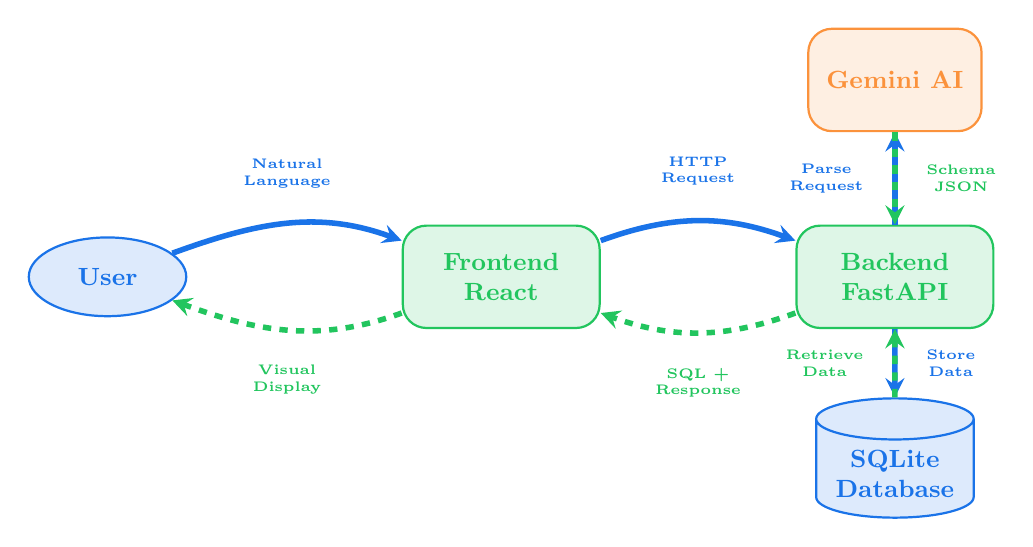
\begin{tikzpicture}[
        node distance=5cm and 4cm,
        auto,
        every node/.style={align=center},
        user/.style={ellipse, draw=primaryblue, fill=primaryblue!15, 
                     minimum width=2cm, minimum height=1cm, 
                     font=\small\bfseries, text=primaryblue, thick},
        process/.style={rectangle, rounded corners=0.3cm, draw=accentgreen, fill=accentgreen!15,
                       minimum width=2.5cm, minimum height=1.3cm,
                       font=\small\bfseries, text=accentgreen, thick},
        ai/.style={rectangle, rounded corners=0.3cm, draw=accentorange, fill=accentorange!15,
                  minimum width=2.2cm, minimum height=1.3cm,
                  font=\small\bfseries, text=accentorange, thick},
        db/.style={cylinder, draw=primaryblue, fill=primaryblue!15, shape border rotate=90, aspect=0.3,
                  minimum width=2cm, minimum height=1.3cm,
                  font=\small\bfseries, text=primaryblue, thick},
        req/.style={->, >=stealth, color=primaryblue, line width=2pt},
        resp/.style={->, >=stealth, color=accentgreen, line width=2pt, dashed}
    ]
        % Place nodes with explicit coordinates for better control
        \node [user] (user) at (0,0) {User};
        \node [process] (frontend) at (5,0) {Frontend\\React};
        \node [process] (backend) at (10,0) {Backend\\FastAPI};
        \node [ai] (ai) at (10,2.5) {Gemini AI};
        \node [db] (db) at (10,-2.5) {SQLite\\Database};
        
        % User <-> Frontend (bidirectional with offset)
        \draw[req] (user) to[out=20,in=160] 
            node[above, midway, font=\tiny\bfseries, yshift=0.3cm] {Natural\\Language} 
            (frontend);
        \draw[resp] (frontend) to[out=200,in=340] 
            node[below, midway, font=\tiny\bfseries, yshift=-0.3cm] {Visual\\Display} 
            (user);
        
        % Frontend <-> Backend (bidirectional with offset)
        \draw[req] (frontend) to[out=20,in=160] 
            node[above, midway, font=\tiny\bfseries, yshift=0.3cm] {HTTP\\Request} 
            (backend);
        \draw[resp] (backend) to[out=200,in=340] 
            node[below, midway, font=\tiny\bfseries, yshift=-0.3cm] {SQL +\\Response} 
            (frontend);
        
        % Backend <-> AI (vertical, clean)
        \draw[req] (backend.north) -- 
            node[left, midway, font=\tiny\bfseries, xshift=-0.25cm] {Parse\\Request} 
            (ai.south);
        \draw[resp] (ai.south) -- 
            node[right, midway, font=\tiny\bfseries, xshift=0.25cm] {Schema\\JSON} 
            (backend.north);
        
        % Backend <-> Database (vertical, clean)
        \draw[req] (backend.south) -- 
            node[right, midway, font=\tiny\bfseries, xshift=0.25cm] {Store\\Data} 
            (db.north);
        \draw[resp] (db.north) -- 
            node[left, midway, font=\tiny\bfseries, xshift=-0.25cm] {Retrieve\\Data} 
            (backend.south);
    \end{tikzpicture}
    }
    
    \vspace{0.3cm}
    \begin{tcolorbox}[colback=lightgray, colframe=primaryblue, boxrule=1.5pt, arc=5pt, 
                     left=8pt, right=8pt, top=6pt, bottom=6pt]
        \centering \small\bfseries 
        \textcolor{primaryblue}{Data Flow:} 
        User Input → Frontend → Backend → AI → Database → Visual Output
    \end{tcolorbox}
\end{frame}

\begin{frame}{Core Operations}
    \begin{enumerate}
        \item \textbf{Natural Language Processing}
        \begin{itemize}
            \item Parse user prompts using Gemini AI
            \item Extract entities, attributes, and relationships
            \item Generate structured JSON schema
        \end{itemize}
        
        \item \textbf{SQL Generation}
        \begin{itemize}
            \item Convert structured schema to CREATE TABLE statements
            \item Apply constraints (PRIMARY KEY, FOREIGN KEY, etc.)
            \item Generate INSERT statements for sample data
        \end{itemize}
        
        \item \textbf{Visual Representation}
        \begin{itemize}
            \item ER diagram view with drag-and-drop
            \item Table view with compact stacking layout
            \item Real-time updates on schema changes
        \end{itemize}
    \end{enumerate}
\end{frame}

\section{Implementation Logic}

\begin{frame}{AI Integration Logic}
    \textbf{Natural Language Parsing Workflow:}
    \begin{enumerate}
        \item Receive and preprocess user prompt
        \item Initialize Gemini AI model with extraction guidelines
        \item Generate structured JSON response
        \item Validate and enhance schema
        \item Return validated schema object
    \end{enumerate}
    
    \vspace{0.3cm}
    \textbf{SQL Generation Logic:}
    \begin{enumerate}
        \item Process each table's columns with data types
        \item Add constraints (PRIMARY KEY, FOREIGN KEY, NOT NULL, UNIQUE)
        \item Format statements according to SQLite syntax
        \item Generate INSERT statements for sample data
    \end{enumerate}
\end{frame}

\begin{frame}{Frontend State Management}
    \begin{columns}
        \column{0.5\textwidth}
        \textbf{State Variables:}
        \begin{itemize}
            \item Entities array
            \item Relationships array
            \item Selected element
            \item SQL code
            \item Table nodes
        \end{itemize}
        
        \column{0.5\textwidth}
        \textbf{Real-Time Updates:}
        \begin{itemize}
            \item Schema changes trigger SQL regeneration
            \item View mode conversion preserves structure
            \item Sample data modifications reflect immediately
        \end{itemize}
    \end{columns}
\end{frame}

\begin{frame}{Data Transformation}
    \textbf{Frontend to Backend:}
    \begin{itemize}
        \item Map entities to tables
        \item Convert attribute IDs to names
        \item Transform sample data keys
        \item Create relationship structure
    \end{itemize}
    
    \vspace{0.3cm}
    \textbf{Backend to Frontend:}
    \begin{itemize}
        \item Reconstruct entities with unique IDs
        \item Convert columns to attributes
        \item Restore attribute positions
        \item Map sample data values back
    \end{itemize}
\end{frame}

\section{Results}

\begin{frame}{System Performance}
    \centering
    \vspace{0.1cm}
    
    \begin{columns}[t]
        \column{0.48\textwidth}
        \begin{tcolorbox}[colback=accentgreen!30, colframe=accentgreen, boxrule=2pt, arc=5pt, left=6pt, right=6pt, top=6pt, bottom=5pt, title=\textbf{84\% Accuracy}]
            \centering
            \vspace{0.05cm}
            \Large \textbf{84\%}
            \vspace{0.05cm}
            
            \footnotesize AI SQL Generation
            
            \vspace{0.05cm}
            \tiny Tested across 50+ queries
        \end{tcolorbox}
        
        \vspace{0.2cm}
        
        \begin{tcolorbox}[colback=accentorange!30, colframe=accentorange, boxrule=2pt, arc=5pt, left=6pt, right=6pt, top=6pt, bottom=5pt, title=\textbf{Response Time}]
            \centering
            \vspace{0.05cm}
            \Large \textbf{2-3s}
            \vspace{0.05cm}
            
            \footnotesize Local Execution
            
            \vspace{0.05cm}
            \tiny Real-time SQL updates
        \end{tcolorbox}
        
        \column{0.48\textwidth}
        \begin{tcolorbox}[colback=primaryblue!30, colframe=primaryblue, boxrule=2pt, arc=5pt, left=6pt, right=6pt, top=6pt, bottom=5pt, title=\textbf{Scalability}]
            \centering
            \vspace{0.05cm}
            \Large \textbf{100+}
            \vspace{0.05cm}
            
            \footnotesize Entities Supported
            
            \vspace{0.05cm}
            \tiny No performance degradation
        \end{tcolorbox}
        
        \vspace{0.2cm}
        
        \begin{tcolorbox}[colback=accentgreen!30, colframe=accentgreen, boxrule=2pt, arc=5pt, left=6pt, right=6pt, top=6pt, bottom=5pt, title=\textbf{Code Quality}]
            \centering
            \vspace{0.05cm}
            \Large \textbf{85\%}
            \vspace{0.05cm}
            
            \footnotesize Test Coverage
            
            \vspace{0.05cm}
            \tiny Unit and integration tests
        \end{tcolorbox}
    \end{columns}
    
    \vspace{0.2cm}
    
    \begin{tcolorbox}[colback=lightgray, colframe=primaryblue, boxrule=1pt, arc=3pt, left=4pt, right=4pt, top=4pt, bottom=4pt]
        \centering \tiny \textbf{Technical Achievements:} Collision-free layout | Dual-view conversion | Schema persistence | Real-time SQL
    \end{tcolorbox}
\end{frame}

\begin{frame}{Validation Results}
    \centering
    \vspace{0.1cm}
    
    \begin{columns}[t]
        \column{0.48\textwidth}
        \begin{tcolorbox}[colback=accentgreen!30, colframe=accentgreen, boxrule=2pt, arc=5pt, left=6pt, right=6pt, top=6pt, bottom=5pt, title=\textbf{User Acceptance}]
            \centering
            \vspace{0.05cm}
            \Large \textbf{25}
            \vspace{0.05cm}
            
            \footnotesize Test Users
            
            \vspace{0.05cm}
            \tiny \textcolor{accentgreen}{\textbf{$\checkmark$}} Positive feedback
            
            \vspace{0.02cm}
            \tiny \textcolor{accentgreen}{\textbf{$\checkmark$}} Intuitive interface
        \end{tcolorbox}
        
        \vspace{0.2cm}
        
        \begin{tcolorbox}[colback=primaryblue!30, colframe=primaryblue, boxrule=2pt, arc=5pt, left=6pt, right=6pt, top=6pt, bottom=5pt, title=\textbf{Testing Coverage}]
            \centering
            \vspace{0.05cm}
            \footnotesize \textbf{Unit:} 85\% coverage
            
            \vspace{0.08cm}
            \footnotesize \textbf{Integration:} All verified
            
            \vspace{0.08cm}
            \footnotesize \textbf{Stress:} 100+ entities
        \end{tcolorbox}
        
        \column{0.48\textwidth}
        \begin{tcolorbox}[colback=accentorange!30, colframe=accentorange, boxrule=2pt, arc=5pt, left=6pt, right=6pt, top=6pt, bottom=5pt, title=\textbf{System Capabilities}]
            \tiny
            \begin{itemize}
                \item[\textcolor{accentorange}{\textbf{•}}] Multiple data types
                \item[\textcolor{accentorange}{\textbf{•}}] Complex ER diagrams
                \item[\textcolor{accentorange}{\textbf{•}}] SQLite DDL generation
                \item[\textcolor{accentorange}{\textbf{•}}] Visual editing
                \item[\textcolor{accentorange}{\textbf{•}}] Real-time updates
                \item[\textcolor{accentorange}{\textbf{•}}] Dual-view switching
            \end{itemize}
        \end{tcolorbox}
        
        \vspace{0.2cm}
        
        \begin{tcolorbox}[colback=lightgray, colframe=primaryblue, boxrule=1pt, arc=3pt, left=4pt, right=4pt, top=4pt, bottom=4pt]
            \centering \tiny \textbf{Status:} \textcolor{accentgreen}{\textbf{$\checkmark$ Tests Pass}} | \textcolor{accentgreen}{\textbf{$\checkmark$ Ready}} | \textcolor{accentgreen}{\textbf{$\checkmark$ Approved}}
        \end{tcolorbox}
    \end{columns}
\end{frame}

\section{Conclusion \& Future Work}

\begin{frame}{Conclusion}
    \textbf{Key Achievements:}
    \begin{itemize}
        \item Successfully integrated AI for natural language to SQL conversion
        \item Developed intuitive visual interface for database design
        \item Implemented robust schema management and persistence
        \item Achieved real-time SQL generation with 2-3s response time (local execution)
    \end{itemize}
    
    \vspace{0.3cm}
    \textbf{Impact:}
    \begin{itemize}
        \item Reduces complexity and time for database schema creation
        \item Makes database design accessible to non-technical users
        \item Provides educational value for learning database concepts
    \end{itemize}
\end{frame}

\begin{frame}{Future Work}
    \vspace{-0.7cm}
    \begin{columns}[t]
        \column{0.5\textwidth}
        \begin{itemize}
            \item[\textcolor{primaryblue}{\large$\bullet$}] \textbf{Multi-Database Support:} 
            Extend beyond SQLite to PostgreSQL, MySQL, and SQL Server with dialect-specific SQL generation
            
            \vspace{0.1cm}
            \item[\textcolor{primaryblue}{\large$\bullet$}] \textbf{AI Model Optimization:} 
            Fine-tune Gemini model for better accuracy, reduce response time, and handle complex queries
            
            \vspace{0.1cm}
            \item[\textcolor{primaryblue}{\large$\bullet$}] \textbf{Advanced Schema Features:} 
            Support CHECK constraints, triggers, indexes, and stored procedures in visual editor
            
            \vspace{0.1cm}
            \item[\textcolor{primaryblue}{\large$\bullet$}] \textbf{Schema Validation \& Suggestions:} 
            AI-powered schema optimization recommendations and automatic constraint validation
        \end{itemize}
        
        \column{0.5\textwidth}
        \begin{itemize}
            \item[\textcolor{accentgreen}{\large$\bullet$}] \textbf{Export \& Import Capabilities:} 
            Export to PDF diagrams, SQL scripts, and import existing database schemas
            
            \vspace{0.1cm}
            \item[\textcolor{accentgreen}{\large$\bullet$}] \textbf{Schema Versioning:} 
            Version control system for schema evolution with rollback capabilities
            
            \vspace{0.1cm}
            \item[\textcolor{accentgreen}{\large$\bullet$}] \textbf{Collaborative Features:} 
            Real-time multi-user editing, comments, and shared workspace functionality
            
            \vspace{0.1cm}
            \item[\textcolor{accentgreen}{\large$\bullet$}] \textbf{Performance Optimization:} 
            Client-side caching, incremental updates, and backend optimization for faster responses
        \end{itemize}
    \end{columns}
\end{frame}

\begin{frame}{Thank You}
    \centering
    \vspace{2cm}
    {\Huge Questions?}
    
    \vspace{1.5cm}
    \textbf{Contact:}
    
    Ankit Kumar \& Rineet Pandey
    
    Department of Computer Science
\end{frame}

\end{document}

